%%
%% This is file `sample-sigconf.tex',
%% generated with the docstrip utility.
%%
%% The original source files were:
%%
%% samples.dtx  (with options: `sigconf')
%% 
%% IMPORTANT NOTICE:
%% 
%% For the copyright see the source file.
%% 
%% Any modified versions of this file must be renamed
%% with new filenames distinct from sample-sigconf.tex.
%% 
%% For distribution of the original source see the terms
%% for copying and modification in the file samples.dtx.
%% 
%% This generated file may be distributed as long as the
%% original source files, as listed above, are part of the
%% same distribution. (The sources need not necessarily be
%% in the same archive or directory.)
%%
%%
%% Commands for TeXCount
%TC:macro \cite [option:text,text]
%TC:macro \citep [option:text,text]
%TC:macro \citet [option:text,text]
%TC:envir table 0 1
%TC:envir table* 0 1
%TC:envir tabular [ignore] word
%TC:envir displaymath 0 word
%TC:envir math 0 word
%TC:envir comment 0 0
%%
%%
%% The first command in your LaTeX source must be the \documentclass command.

%, anonymous
\documentclass[sigconf]{acmart}
\usepackage[portuguese]{babel}
\usepackage{listings}
\usepackage{xcolor}
\usepackage{hyperref}
\usepackage{tabularx}
\usepackage[boxruled, linesnumbered]{algorithm2e}
\usepackage{geometry}
\usepackage{amsmath}

\definecolor{dkgreen}{rgb}{0,0.6,0}
\definecolor{gray}{rgb}{0.5,0.5,0.5}
\definecolor{mauve}{rgb}{0.58,0,0.82}


\lstset{frame=tb,
  language=Java,
  showstringspaces=false,
  columns=flexible,
  basicstyle={\small\ttfamily},
  numbers=left,
  numberstyle=\tiny\color{gray},
  keywordstyle=\color{blue},
  commentstyle=\color{dkgreen},
  stringstyle=\color{mauve},
  breaklines=true,
  breakatwhitespace=true,
  tabsize=3,
  literate={á}{{\'a}}1 {ã}{{\~a}}1 {é}{{\'e}}1
}

\newcommand{\rev}[1]{\textcolor{black}{#1}}

%%
%% \BibTeX command to typeset BibTeX logo in the docs
\AtBeginDocument{%
  \providecommand\BibTeX{{%
    \normalfont B\kern-0.5em{\scshape i\kern-0.25em b}\kern-0.8em\TeX}}}

%% Rights management information.  This information is sent to you
%% when you complete the rights form.  These commands have SAMPLE
%% values in them; it is your responsibility as an author to replace
%% the commands and values with those provided to you when you
%% complete the rights form.
\setcopyright{acmcopyright}
\copyrightyear{2022}
\acmYear{2022}
\acmDOI{XXXXXXX.XXXXXXX}

%% These commands are for a PROCEEDINGS abstract or paper.
\acmConference[XXXVI Simpósio Brasileiro de Engenharia de Software]{}{Uberlândia, MG}{3 a 7 de outubro}
%\acmPrice{15.00}
%\acmISBN{978-1-4503-XXXX-X/18/06}


%%
%% Submission ID.
%% Use this when submitting an article to a sponsored event. You'll
%% receive a unique submission ID from the organizers
%% of the event, and this ID should be used as the parameter to this command.
%%\acmSubmissionID{123-A56-BU3}

%%
%% The majority of ACM publications use numbered citations and
%% references.  The command \citestyle{authoryear} switches to the
%% "author year" style.
%%
%% If you are preparing content for an event
%% sponsored by ACM SIGGRAPH, you must use the "author year" style of
%% citations and references.
%% Uncommenting
%% the next command will enable that style.
%%\citestyle{acmauthoryear}

%%
%% end of the preamble, start of the body of the document source.
\begin{document}

%%
%% The "title" command has an optional parameter,
%% allowing the author to define a "short title" to be used in page headers.
\title{Detecção de conflitos semânticos via análise estática de substituição de atribuição}

%%
%% The "author" command and its associated commands are used to define
%% the authors and their affiliations.
%% Of note is the shared affiliation of the first two authors, and the
%% "authornote" and "authornotemark" commands
%% used to denote shared contribution to the research.


\author{Matheus Barbosa}
\affiliation{%
    \institution{Centro de Informática}
    \institution{Universidade Federal de Pernambuco}
}
\email{mbo2@cin.ufpe.br}

\author{Paulo Borba}
\affiliation{%
    \institution{Centro de Informática}
    \institution{Universidade Federal de Pernambuco}
}
\email{phmb@cin.ufpe.br}

\author{Rodrigo Bonifacio}
\affiliation{%
  \institution{Universidade de Brasilia}
}
\email{rbonifacio@unb.br}

\author{Galileu Santos}
\affiliation{%
  \institution{Centro de Informática}
 \institution{Universidade Federal de Pernambuco}
}
\email{gsj@cin.ufpe.br}


%%
%% By default, the full list of authors will be used in the page
%% headers. Often, this list is too long, and will overlap
%% other information printed in the page headers. This command allows
%% the author to define a more concise list
%% of authors' names for this purpose.


%%
%% The abstract is a short summary of the work to be presented in the
%% article.
%%Normalmente os desenvolvedores trabalham de forma colaborativa e com frequência precisam incorporar seus códigos a uma versão principal do sistema. Esse processo pode ocasionar conflitos de \emph{merge}, afetando a produtividade da equipe. Alguns desses conflitos requerem a compreensão do comportamento do \emph{software} (conflitos semânticos) e não podem ser detectados ferramentas atuais de controle de versão. Desta forma, se faz necessário ferramentas que possam detectar conflitos semânticos no processo de integração. Esse trabalho propõe uma análise de substituição de atribuição (\emph{Override an Assignment (OA)}), que visa detectar interferências entre as alterações introduzidas por dois desenvolvedores diferentes, onde caminhos de gravação, sem atribuições intermediárias, para um alvo comum indicam interferência. Para avaliar as implementações da análise proposta foi usado um conjunto de 78 cenários de integração de código. Os resultados mostram que a análise proposta consegue detectar cenários com substituições de atribuições e com interferência localmente observável entre as contribuições.
\begin{abstract}
Developers typically work collaboratively and often need to embed their code into a major version of the system. This process can cause \emph{merge} conflicts, affecting team productivity. Some of these conflicts require understanding \emph{software} behavior (semantic conflicts) and current version control tools are not able to detect that. So here we explore how such conflicts could be automatically detected using static analysis of the integrated code. We propose and implement an assignment overriding analysis, which aims to detect interference between changes introduced by two different developers, where write paths, without intermediate assignments, to a common target indicate interference. To evaluate the implementations of the proposed analysis, a set of 78 code integration scenarios was used. The results show that the proposed analysis is able to detect scenarios with assignment overriding and with locally observable interference between the contributions.
\end{abstract}

%%
%% The code below is generated by the tool at http://dl.acm.org/ccs.cfm.
%% Please copy and paste the code instead of the example below.
%%
\begin{CCSXML}
<ccs2012>
 <concept>
  <concept_id>10010520.10010553.10010562</concept_id>
  <concept_desc>Computer systems organization~Embedded systems</concept_desc>
  <concept_significance>500</concept_significance>
 </concept>
 <concept>
  <concept_id>10010520.10010575.10010755</concept_id>
  <concept_desc>Computer systems organization~Redundancy</concept_desc>
  <concept_significance>300</concept_significance>
 </concept>
 <concept>
  <concept_id>10010520.10010553.10010554</concept_id>
  <concept_desc>Computer systems organization~Robotics</concept_desc>
  <concept_significance>100</concept_significance>
 </concept>
 <concept>
  <concept_id>10003033.10003083.10003095</concept_id>
  <concept_desc>Networks~Network reliability</concept_desc>
  <concept_significance>100</concept_significance>
 </concept>
</ccs2012>
\end{CCSXML}

%%
%% Keywords. The author(s) should pick words that accurately describe
%% the work being presented. Separate the keywords with commas.

%%
%% This command processes the author and affiliation and title
%% information and builds the first part of the formatted document.
\maketitle

\section{Introdução}
O processo de desenvolvimento de \emph{software} atual, exceto em casos especiais, é feito de forma colaborativa. Em um ambiente colaborativo, é comum que vários desenvolvedores estejam trabalhando em seus ramos individuais (\emph{branches}) simultaneamente, e com frequência incorporem seus códigos a uma versão principal do sistema. No entanto, na prática, o processo de integração de alterações de ramos múltiplos pode ser difícil e propenso a erros, especialmente se as alterações em diferentes ramos entrarem em conflito \cite{Bird2012AssessingTV}, afetando a produtividade da equipe \cite{6915251}.

Alguns desses conflitos requerem a compreensão do comportamento do \emph{software} (conflitos semânticos), e não podem ser detectados por ferramentas atuais de \emph{Merge} como o diff3 \cite{10.5555/1781794.1781836}, podendo levar à introdução de bugs no código, influenciando negativamente na qualidade do produto final.  Horwitz et al.~\cite{Horwitz1989IntegratingNV} especificaram formalmente os conflitos semânticos: duas contribuições advindas de versões \emph{Left} e \emph{Right} para um programa \emph{Base}, originam um conflito semântico se as especificações que as versões se propõem a cumprir em isolado não são satisfeitas na versão integrada \emph{Merge}.\footnote{Versões envolvidas em um \emph{three-way merge}, onde \emph{Base} é o ancestral comum mais recente às duas versões \emph{Left} e \emph{Right}} 
Na prática, não é possível checar a existência dos conflitos semânticos, pois não temos as especificações e não sabemos a intenção real dos desenvolvedores.

Algumas abordagens diferentes já foram utilizadas, como, por exemplo, geração de testes \cite{LeusonSilva2020}. Porém,
essas tendem a apresentar um número alto de falsos negativos, pois verificam se há interferência a partir de valores específicos na execução do código testado.

Também já foram propostos algoritmos de análise estática para detecção de conflitos semânticos  \cite{InformationFlowRoberto, Binkley95programintegration, Horwitz1989IntegratingNV}, mas esses são baseados em grafos complexos (\emph{System Dependence Graphs} \cite{Horwitz1989IntegratingNV}), e à medida que as bases de código aumentam, têm a performance bastante degradada, o que torna essas soluções difíceis de serem aplicadas em bases de código reais de mais de 50 KLOC \cite{InformationFlowRoberto}. Diante disso, surge a necessidade de explorar simplificações dos algoritmos originalmente propostos, de modo a verificar a sua capacidade de detectar os conflitos semânticos com menor custo computacional.

Dessa forma, neste trabalho \rev{implementamos e avaliamos um tipo específico de análise estática para detectar interferências}\footnote{Para detectarmos conflitos, precisaríamos saber a intenção dos desenvolvedores, pois assumimos um conflito como sendo uma interferência não intencional entre mudanças integradas dos desenvolvedores. Desta forma, buscamos detectar uma interferência que é quando o comportamento das mudanças integradas não preserva a intenção das mudanças individuais. Esse trabalho usa o conceito de interferência como aproximação para conflito por não ser possível inferir as intenções dos desenvolvedores.} entre as alterações introduzidas por dois desenvolvedores diferentes, através de uma análise de substituição de atribuição (OA). Consideramos que pode haver OA quando as alterações (adições e modificações) em um dos ramos podem semanticamente (ou seja, sua execução), envolver uma operação de escrita para um elemento de estado que também está associado a uma operação de escrita envolvida nas alterações (adições e modificações) feitas pelo outro ramo, sem operação de escrita da base entre eles.

Para melhor entender o compromisso entre acurácia e eficiência de OA, implementamos uma versão \emph{intraprocedural}, que desconsidera chamadas de método no código analisado e outra \emph{interprocedural}, que  acessa e analisa o corpo das chamadas de método no código analisado.

As implementações da análise proposta (\emph{intraprocedural} e \emph{interprocedural}) foram avaliadas usando um conjunto de 78 cenários de integração de código. Esses cenários foram extraídos de projetos \emph{open-source} Java.

Para cada um dos cenários utilizados foi realizada uma validação manual estruturada para definir o \emph{ground truth} de interferência localmente observável (LOI). Os resultados da execução das análises foram comparados com o \emph{ground truth} para verificar a capacidade das análises em detectar interferências. Por fim, também foram coletadas métricas de precisão, revocação e acurácia usadas para comparar as implementações \emph{intraprocedural} e \emph{interprocedural}. Adicionalmente, também realizamos uma comparação dos resultados com um \emph{ground truth} de OA, buscando identificar o quão próximo as implementações atuais estão de uma implementação ideal.    

Os resultados apontam que as implementações da análise proposta se mostraram capazes de detectar cenários com interferência entre as contribuições, no entanto, teve uma quantidade considerável de falsos negativos. Isso indica que ela não é suficiente para detectar cenários com interferência de forma confiável. Portanto, a análise proposta poderia ser combinada com outras análises para compor uma ferramenta mais robusta para detecção de conflitos de integração semânticos. 
\section{Motivação e Conceitos Básicos}
\subsection{Caso Motivador}
Para exemplificar melhor o conceito de conflito de integração semântico, considere o cenário de exemplo da \hyperref[fig:codigo-motivador]{Figura 1}.\footnote{Assumindo um cenário de \emph{merge} formado por \emph{commits Base, Left, Right e Merge}, esse último contendo o arquivo apresentado na figura.} Conseguimos observar a classe \texttt{Text}, que contém três atributos: uma \emph{string}, que referencia o texto representado pelos objetos dessa classe e dois atributos do tipo inteiro, que correspondem à quantidade de correções aplicadas ao texto (remoção de espaços e palavras duplicadas), e a quantidade de comentários no texto. A classe \texttt{Text} também conta com o método \texttt{generateReport()} responsável por gerar o relatório da quantidade de \texttt{fixes} necessárias e comentários existentes.

Na \hyperref[fig:codigo-motivador]{Figura 1} é exibido o arquivo resultado da integração das mudanças em amarelo (Linha 6 foi adicionada pela versão \emph{Left}) e as mudanças em verde (Linha 8 foi adicionada pela versão \emph{Right}). As outras linhas de código são de uma versão \emph{Base}, o ancestral comum mais recente de ambas versões \emph{Left} e \emph{Right}\footnote{Para simplificar, assumimos um único ancestral comum (mais recente). As situações de \emph{Merge} cruzado no git, pode haver mais de um}. Nesse caso, podemos observar que as mudanças adicionadas por \emph{Left} e \emph{Right} não estão na mesma linha e nem em linhas consecutivas, assim as alterações podem ser \emph{textualmente} integradas com segurança e nenhum conflito seria reportado pelas ferramentas de \emph{Merge} atuais. 

\begin{figure}[!h]
    \begin{lstlisting}[escapechar=!]
    class Text {
        public String text;
        public int fixes;
        public int comments;
        void generateReport() {
+           !\colorbox{yellow}{countDuplicatedWhitespaces();}!
            countComments();
+           !\colorbox{green}{countDuplicatedWords();}!
        }
    }
    \end{lstlisting}
    \caption{Caso de exemplo de conflito integração semântico}
    \label{fig:codigo-motivador}
\end{figure}

Observando um pouco melhor as alterações de cada um dos desenvolvedores, assuma que \emph{Left}, ao adicionar a chamada do método \texttt{countDuplicatedWhitespaces()}, pretende realizar a contagem dos espaços em branco em um determinado texto e, ao final, sobrescreve o atributo \texttt{fixes} com o valor da contagem. Já \emph{Right}, adicionou a chamada ao método \texttt{countDuplicatedWords()} que sobrescreve \texttt{fixes} com o valor da contagem das palavras duplicadas no determinado texto. Entre as alterações de \emph{Left} e \emph{Right} temos um comando que vem de \emph{Base}. A chamada ao método \texttt{countComments()} realiza a contagem dos comentários no atributo \texttt{text}, mas diferente das demais chamadas de métodos, altera o atributo \texttt{comments}.

Apesar de a integração ter gerado um código sintaticamente válido e livre de conflitos textuais, a mudança feita por \emph{Right} interfere com a mudança feita por \emph{Left}, já que a execução da chamada ao \texttt{countDuplicateWords()} altera o valor do atributo \texttt{fixes}, que também é alterado pela chamada ao \texttt{countDuplicateWhitespace()}. Considerando que a intenção ou especificação da tarefa de \emph{Left} era exatamente armazenar em \texttt{fixes} a quantidade de espaços duplos, e que isso não acontece ao final da execução de \texttt{generateReport()}, quando \texttt{fixes} estará armazenando o número de palavras duplicadas, teremos então, um conflito semântico.\footnote{Mesmo que a implementação fosse outra, os resultados (de OA, conflito, interferência) poderiam ser os mesmos, assumindo especificações óbvias para o caso e o não conhecimento mútuo das tarefas de \emph{Left} e \emph{Right}} 

Em particular, a mudança feita por \emph{Right} inadvertidamente anula a mudança feita por \emph{Left}.
Para entender melhor porque há interferência nesse caso, considere o caso de teste ilustrado na \hyperref[fig:teste-motivador]{Figura 2}, escrito por \emph{Left} para confirmar que sua tarefa foi corretamente implementada.

\begin{figure}[h]
    \begin{lstlisting}[]
    public void countFixesTest() throws Throwable {
        Text t = new Text();
        t.text = "the the     dog dog";
        t.generateReport();
        assertTrue(1, t.fixes);
    }
    \end{lstlisting}
    \caption{Caso de teste que demonstra o conflito semântico na Figura 2.1}
    \label{fig:teste-motivador}
\end{figure}

O caso de teste executa o método \texttt{t.generateReport()}, utilizando como \emph{String} de entrada \texttt{‘‘the the\quad dog dog’’}. Se executarmos esse teste apenas na versão de \emph{Left} (sem a linha 8 Verde), o teste passará, pois existe apenas um espaço em branco no texto (entre as palavras \texttt{the} e \texttt{dog}). Já executando apenas no ramo de \emph{Right} (sem a linha 6 amarela) o teste falhará, pois \texttt{‘‘the the’’} e \texttt{‘‘dog dog’’} somam duas palavras duplicadas. Agora pensando apenas no cenário de \emph{merge} (\hyperref[fig:codigo-motivador]{Figura 1}) o teste também irá falhar, pois o último método a ser chamado é o \texttt{countDuplicatedWords()} adicionado por \emph{Right}, que sobrescreve \texttt{fixes} com o valor da quantidade de palavras duplicadas no texto.

Em isolado, ambos desenvolvedores implementaram suas tarefas corretamente, cumprindo os contratos que pretendiam. No entanto, devido a um detalhe da implementação adicionada pela versão \emph{Right}, o código integrado não cumpre o contrato pretendido pelo desenvolvedor de \emph{Left} (\texttt{fixes} deveria ser igual a 1). Perceba que a intenção de um dos desenvolvedores (\emph{Left}) não é preservada no \emph{merge}, ocorrendo assim uma interferência. 

Casos como esse, são muitas vezes difíceis e caros de se detectar e resolver. Na verdade, exceto em projetos que adotem boas práticas de escrita de código, práticas de revisão e tenha conjuntos de testes fortes, espera-se que a maioria dos conflitos semânticos escapem para os usuários. Mesmo com tais práticas, conflitos semânticos ainda são esperados. Se a detecção não for imediata após integração, pode ser ainda mais difícil corrigi-los, pois a resolução envolve a reconciliação da incompatibilidade semântica comportamental \cite{LeusonSilva2020}. Em nosso exemplo, teríamos que investigar se o defeito está nas implementações individuais de \emph{Left} e \emph{Right} ou em como um deles interfere no outro. Isto exigiria uma investigação não superficial que quebrasse os limites da abstração estabelecidos pelas declarações dos métodos chamados em \texttt{generateReport()}.

Para evitar esses problemas mencionados, bastaria executar a análise de substituição de atribuição proposta. No caso específico, nossa implementação detecta essa interferência, pois a análise de OA busca por alterações feitas por desenvolvedores diferentes, e que durante a execução, escrevem no mesmo componente do estado (\texttt{fixes}), sem atribuições intermediárias. De fato, a atribuição feita por \texttt{countDuplicateWhitespace()} em \texttt{fixes} é sobrescrita pela atribuição feita por \texttt{countDuplicatedWords()} e \texttt{countComments()} escreve em \texttt{comments}, não interferindo em \texttt{fixes}. 


\begin{figure}[!h]
    \begin{lstlisting}[escapechar=!]
right no método Text.countDuplicatedWords na linha 8, atribui o valor 2 a variável fixes e interfere em left no método Text.countDuplicatedWhitespaces na linha 6 que atribuiu o valor 1 para variável fixes.
    \end{lstlisting}
    \caption{Exemplo simplificado de um alerta reportado pela análise proposta}
    \label{fig:report-caso-motivador}
\end{figure}

Na \hyperref[fig:report-caso-motivador]{Figura 3}, temos um exemplo simplificado de um alerta reportado pela análise proposta.\footnote{Este é um exemplo simplificado para fins didáticos. A saída da ferramente pode ser um pouco diferente.} Os detalhes contêm a classe, o método, o número da linha e a instrução em que a substituição de atribuição aconteceu.

\subsection{Conceitos Básicos}

A definição de interferência localmente observável é inspirada na definição dada por Horwitz et al. \cite{Horwitz1989IntegratingNV}, que definiu um conflito de integração semântico como um cenário em que as contribuições das versões interferem entre si. Para ajudar a compreender melhor as definições que utilizamos neste trabalho, podemos observar a imagem ilustrada na  \hyperref[fig:analysis]{Figura 4}. Implementamos duas abordagens para detecção de OA em cenários de integração de código. OA \emph{intraprocedural} e OA \emph{interprocedural} são implementações que tentam ao máximo, dentro de suas características, uma aproximação para a definição da análise de substituição de atribuição OA. No que lhe concerne, OA é um tipo de interferência que busca identificar atribuições de dois desenvolvedores na mesma variável e atributos. Neste trabalho, utilizamos as interferências localmente observáveis, pois é a categoria de interferência que facilita a avaliação manual. Por fim, temos o conceito de interferência como aproximação para conflito, pois um conflito nada mais é do que interferência não intencional entre mudanças integradas dos desenvolvedores.

\begin{figure}[!h]
    \centering
    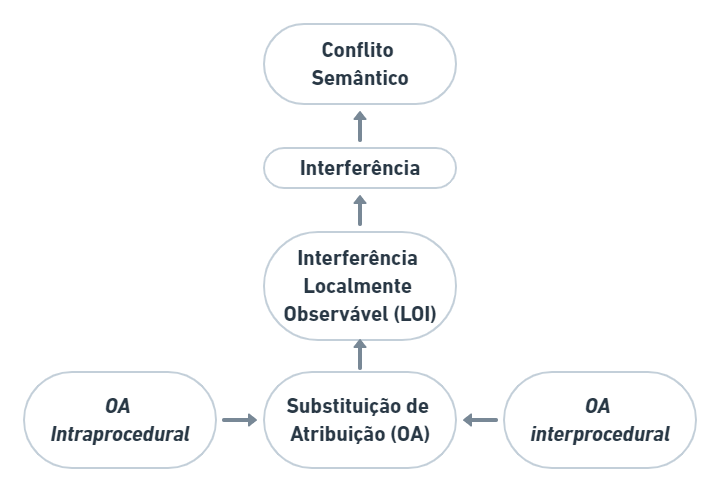
\includegraphics[width=0.8\linewidth]{images/analysis.png}
    \caption{Representação da hierarquia da análise até o conflito semântico}
    \label{fig:analysis}
\end{figure}

É importante ressaltar que OA e LOI são independentes, ou seja, para que um exista não é necessária a existência do outro.

Um exemplo de caso em que existe OA, mas não existe LOI, pode ser observado na imagem da \hyperref[fig:f3d6309]{Figura 5}. Não há LOI, pois \emph{Right} fez uma refatoração (\emph{extract variable} na variável \texttt{json}). No entanto, existe OA, pois os dois desenvolvedores atribuem a variável \texttt{setings}.

\begin{figure}[!h]
    \begin{lstlisting}[escapechar=!]
    public void testQueryModeCommonGramsAnalysis() {
       !\colorbox{yellow}{String json = "/org/elasticsearch/..."}!
        Settings settings = Settings.settingsBuilder()
            .loadFrom!\colorbox{yellow}{Stream(json, ...)}!
            .put("path.home", create!\colorbox{green}{Home}!())
            .build();
        }
    \end{lstlisting}
    \caption{Adaptação do Arquivo de \emph{merge} do cenário f3d6309 como exemplo de OA sem LOI}
    \label{fig:f3d6309}
\end{figure}

Para os casos em que não existe OA, mas existe LOI, temos o exemplo ilustrado na \hyperref[fig:3d4f995]{Figura 6}. Existe LOI, pois \emph{Right} está usando uma variável (\texttt{oplogDb}) alterada por \emph{Left}. Não existe OA, pois os desenvolvedores não sobrescrevem a mesma variável em nenhum momento.

\begin{figure}[!h]
    \begin{lstlisting}[escapechar=!]
    ...
    !\colorbox{yellow}{oplogDb = oplogDb.getMongo().getDB(...);}!
    ...
    !\colorbox{green}{oplogRefsCollection = oplogDb.getCollection(...);}!
    ...
    \end{lstlisting}
     \caption{Adaptação do arquivo de \emph{merge} do cenário 3d4f995 como exemplo de LOI sem OA}
    \label{fig:3d4f995}
\end{figure}
\section{Análise de substituição de atribuição (OA)}

A análise proposta, essencialmente, verifica se a execução das mudanças feitas por um desenvolvedor (digamos, \emph{Left}), pode sobrescrever uma atribuição (OA) da execução das mudanças feitas pelo outro desenvolvedor (digamos, \emph{Right}), ou vice-versa.

Consideramos que pode haver OA quando as alterações (adições e modificações) em um dos ramos podem semanticamente (ou seja, sua execução), envolver uma operação de escrita para um elemento de estado\footnote{Variável local, parâmetro, campo estático ou de instância, arquivo, fluxo, expressão na instrução de retorno, exceção levantada, etc. Incluindo o estado temporário também. Por exemplo, no código ilustrado na \hyperref[fig:codigo-motivador]{Figura 1} tem como elementos de estado os atributos \texttt{text}, \texttt{fixes} e \texttt{comments}}, que também estão associados a uma operação de escrita envolvida nas alterações (acréscimos e modificações) feitas por outro ramo e não há operação de escrita entre eles. 

Como vimos na seção anterior, o exemplo da \hyperref[fig:codigo-motivador]{Figura 1} contém uma interferência. Como essa interferência não foi planejada, podemos afirmar que se trata de um conflito semântico. Agora, imagine que a chamada ao método \texttt{countComments()} também sobrescrevesse a variável \texttt{fixes}. Com isso, não existiria interferência entre \emph{Right} e \emph{Left}. Resumidamente, \emph{Right} não estaria sobrescrevendo uma variável alterada por \emph{Left} e sim por \emph{Base}, o que não ocasiona conflitos semânticos.

Seguindo o mesmo raciocínio, as referências a atributos de um objeto como \texttt{o.a} e \texttt{o.b} são consideradas diferentes elementos de estado e podem ser escritas pelas ramificações sem levar à interferência. Por outro lado, a variável \texttt{o} também representa um elemento de estado diferente, mas não pode ser alterado junto com \texttt{o.a} ou \texttt{o.b} sem causar interferência. (\hyperref[fig:object-samples]{Figura 7}).


\begin{figure}[h]
    \begin{lstlisting}[escapechar=!]
    void m() { // Sem Interferencia
        Object o = new Object();
+       !\colorbox{yellow}{o.a = "exemplo A";}!
        ...
+       !\colorbox{green}{o.b = "exemplo B";}!
    }
    void m() { // Com Interferencia
        Object o = new Object();
+       !\colorbox{yellow}{o = new Object();}!
        ...
+       !\colorbox{green}{o.a = "exemplo";}!
    }
    \end{lstlisting}
    \caption{Caso de exemplo com objetos}
    \label{fig:object-samples}
\end{figure}

Algo similar acontece com \emph{arrays}, onde cada posição corresponde a um elemento de estado diferente. Dessa forma, \texttt{a[0]} e \texttt{a[1]} podem ser escritos por versões de desenvolvedores diferentes e isso não leva à interferência. No entanto, a variável \texttt{a} corresponde a um elemento de estado diferente, mas não pode ser alterado junto com \texttt{a[0]} e \texttt{a[1]} sem causar interferência.

Outro detalhe importante é com relação à acurácia com que a análise detecta interferência. A análise proposta é considerada conservadora. Para exemplificar isso, podemos imaginar uma versão da \hyperref[fig:codigo-motivador]{Figura 1}, em que a atribuição do desenvolvedor \emph{Right} está no escopo de um comando condicional \texttt{if}. Por se tratar de uma análise estática, em casos como esse, a análise não conseguiria inferir se a condição do \texttt{if} seria verdadeira ou falsa, Dessa forma, a análise irá verificar as duas possibilidades, o que resultaria em interferência para esse exemplo, mesmo que a condição do \texttt{if} nunca viesse a ser \emph{true} em execuções do sistema.

\subsection{Especificação do Algoritmo}

Um pseudocódigo simplificado do algoritmo pode ser observado na imagem a seguir.

\begin{algorithm}[h]
    \caption{Algoritmo de substituição de atribuição}
    
    \SetKwInOut{Input}{input}
    \SetKwInOut{Output}{output}

    \Input{Um método de entrada $m$}
    \Output{Uma lista de interferências}
    
    \SetKwData{abstractionRight}{abstractionRight}\SetKwData{abstractionLeft}{abstractionLeft}
   
    \SetKwProg{Fn}{}{\string:}{end}
    \SetKwFunction{traverse}{traverse}
    \SetKwFunction{isTagged}{isTagged}
    \SetKwFunction{isAssigment}{isAssigment}
    \SetKwFunction{isRight}{isRight}
    \SetKwFunction{isLeft}{isLeft}
    \SetKwFunction{isMethodCall}{isMethodCall}
    \SetKwFunction{checkConflict}{checkConflict}
    \SetKwFunction{kill}{kill}
    
    \BlankLine
    \Fn{\traverse($m$)}{
        \ForEach{$cmd\in m$}{
            \uIf{\isTagged($cmd$)}{
                \uIf{\isAssigment($cmd$)}{
                    \uIf{\isRight($cmd$)}{
                        $abstractionRight\leftarrow cmd$\
                    }
                    \uElseIf{\isLeft($cmd$)}{
                        $abstractionLeft\leftarrow cmd$\;
                    }
                    \tcc*[h]{verifica se existe Interferência e adiciona na lista de conflitos}
                    
                    \checkConflict($cmd$)\;
                }
                \uElseIf{\isMethodCall($cmd$)}{
                    \traverse($cmd$)\;
                }
            }
            \Else{
                \tcc*[h]{remove o comando das listas.}
                
                \kill($cmd$)\; 
            }
        }
    }
\end{algorithm}


De modo geral, o algoritmo da análise proposta consiste em percorrer os comandos de um método de entrada.\footnote{A implementação atual considera como método de entrada o método onde ocorreu a primeira modificação feita pelo desenvolvedor \emph{Left}} Quando encontra uma atribuição adicionada por \emph{Left} ou \emph{Right}, guarda essa informação em um conjunto que contém os elementos do estado alterado.\footnote{Tal conjunto corresponde a uma abstração na infraestrutura de análise de programas \emph{Soot Framework}. Outro termo comumente encontrado na literatura é \emph{lattice}.} Uma interferência é reportada sempre que o elemento de estado já existe no conjunto. Quando encontra uma atribuição de \emph{Base}, tira do conjunto. Para \emph{interprocedural}, adicionalmente atravessa recursivamente os comandos do método chamado quando encontra uma chamada de método.

Neste trabalho, implementamos duas abordagens diferentes: (\emph{intraprocedural} e \emph{interprocedural}) para a análise de substituição de atribuição proposta.

\subsubsection*{Análise intraprocedural}

A implementação \emph{intraprocedural} é mais barata com relação aos custos computacionais, assim, não consegue detectar interferências quando ocorrem em métodos chamados a partir do método de entrada, pois desconsidera comandos de chamada de método, não alterando a abstração da análise e seguindo para o próximo comando.

\subsubsection*{Análise interprocedural}

A implementação \emph{interprocedural} é mais robusta e, consequentemente, mais cara. Quando a análise \emph{interprocedural} recebe um comando de chamada de método, ela recupera o corpo do método que está sendo chamado e o analisa, eventualmente alterando a abstração da análise, para só depois voltar para analisar o próximo comando. 


\subsection{Implementação}
As abordagens da análise proposta foram implementadas utilizando a linguagem de programação Java e a \emph{API} do \emph{Soot Framework}\footnote{http://soot-oss.github.io/soot/} para executar o algoritmo descrito anteriormente.\footnote{As implementações da análise proposta pode ser encontrada no repositório \href{https://github.com/spgroup/conflict-static-analysis}{https://github.com/spgroup/conflict-static-analysis}. Este projeto, disponível no \emph{Github}, reúne as implementações utilizadas para esse e outros trabalhos e visa implementar uma biblioteca de análises estáticas para detectar conflitos de merge semântico.} 

As análises recebem como entrada o código compilado da versão integrada empacotado em um arquivo \emph{.JAR} e um arquivo \emph{.CSV} gerado pela ferramenta \emph{miningframework}\footnote{Um framework para mineração de projetos git. \href{https://github.com/spgroup/miningframework}{https://github.com/spgroup/miningframework}}, em que cada linha representa uma linha de código modificada\footnote{Para esse trabalho, as linhas de código deletadas não são coletadas, pois, a análise de substituição de atribuição proposta não as considera. As linhas removidas são consideradas para análise manual de interferência.}, contendo as informações do nome da classe modificada e o número da linha modificada para a versão integrada, e se essa linha foi modificada por \emph{Left} ou \emph{Right}.
\section{Avaliação}

As seções a seguir descrevem a metodologia utilizada para compreender as implicações do uso da abordagem proposta na identificação de conflitos semânticos. Além disso, verificamos o quão perto as nossas implementações atuais da análise estão perto de uma implementação ideal de OA. Fazemos também uma breve comparação do desempenho das implementações. Por fim, apresentamos os resultados obtidos e às ameaças a validade.

\subsection{Dataset}
Para avaliar a capacidade da análise proposta de detectar interferência entre as contribuições de diferentes versões, foi utilizado um conjunto de dados com 78 cenários de integração de projetos \emph{open-source} Java extraídos do \emph{Github}. \rev{Cada um desses cenários contém um método ou campo de uma classe modificado em ambas versões Left e Right --- isto é, os ramos integrados em uma determinada operação de merge.} Esse tipo de cenário em específico foi escolhido, pois são mais suscetíveis a ocorrência de interferência. Alguns desses cenários foram aproveitados de outros trabalhos relacionados, sendo 5 de Da Silva et. al. \cite{LeusonSilva2020}, 19 de Barros Filho  \cite{InformationFlowRoberto}, 26 de De Souza et. al. \cite{10.1145/958160.958177} e 7 de Cavalcanti et. al. \cite{10.1109/ASE.2019.00097}. Os outros 21 cenários foram minerados a partir de uma lista de projetos \emph{open-source} populares utilizando o \emph{miningframework}. \rev{A lista com todos os cenários e projetos utilizados pode ser encontrada no Apêndice online \rev{\cite{sitesbes2022}}.}

O processo de coleta dos dados utilizados é ilustrado pela \hyperref[fig:mineracao]{Figura 8}. A ferramenta de mineração recebe como entrada um arquivo com uma lista de repositórios no \emph{Github} e cria \emph{forks} dos repositórios para configurar uma ferramenta de CI (Integração Contínua). Logo após o \emph{miningframework} cria o cenário contendo os arquivos das versões \emph{Base}, \emph{Left} e \emph{Right} que serão utilizados para coletar as linhas modificadas por cada um dos desenvolvedores. Em seguida, a ferramenta executa o processo descrito na caixa tracejada para cada um dos \emph{commits} de \emph{merge} envolvido no \emph{three-way merge}\footnote{Um  \emph{three-way merge} acontece quando dois conjuntos de alterações em um arquivo base são integrados à medida que são aplicados, em vez de aplicar um e, em seguida, integrar o resultado com o outro.} dos projetos passados como entrada. 

\begin{figure}[!h]
    \centering
    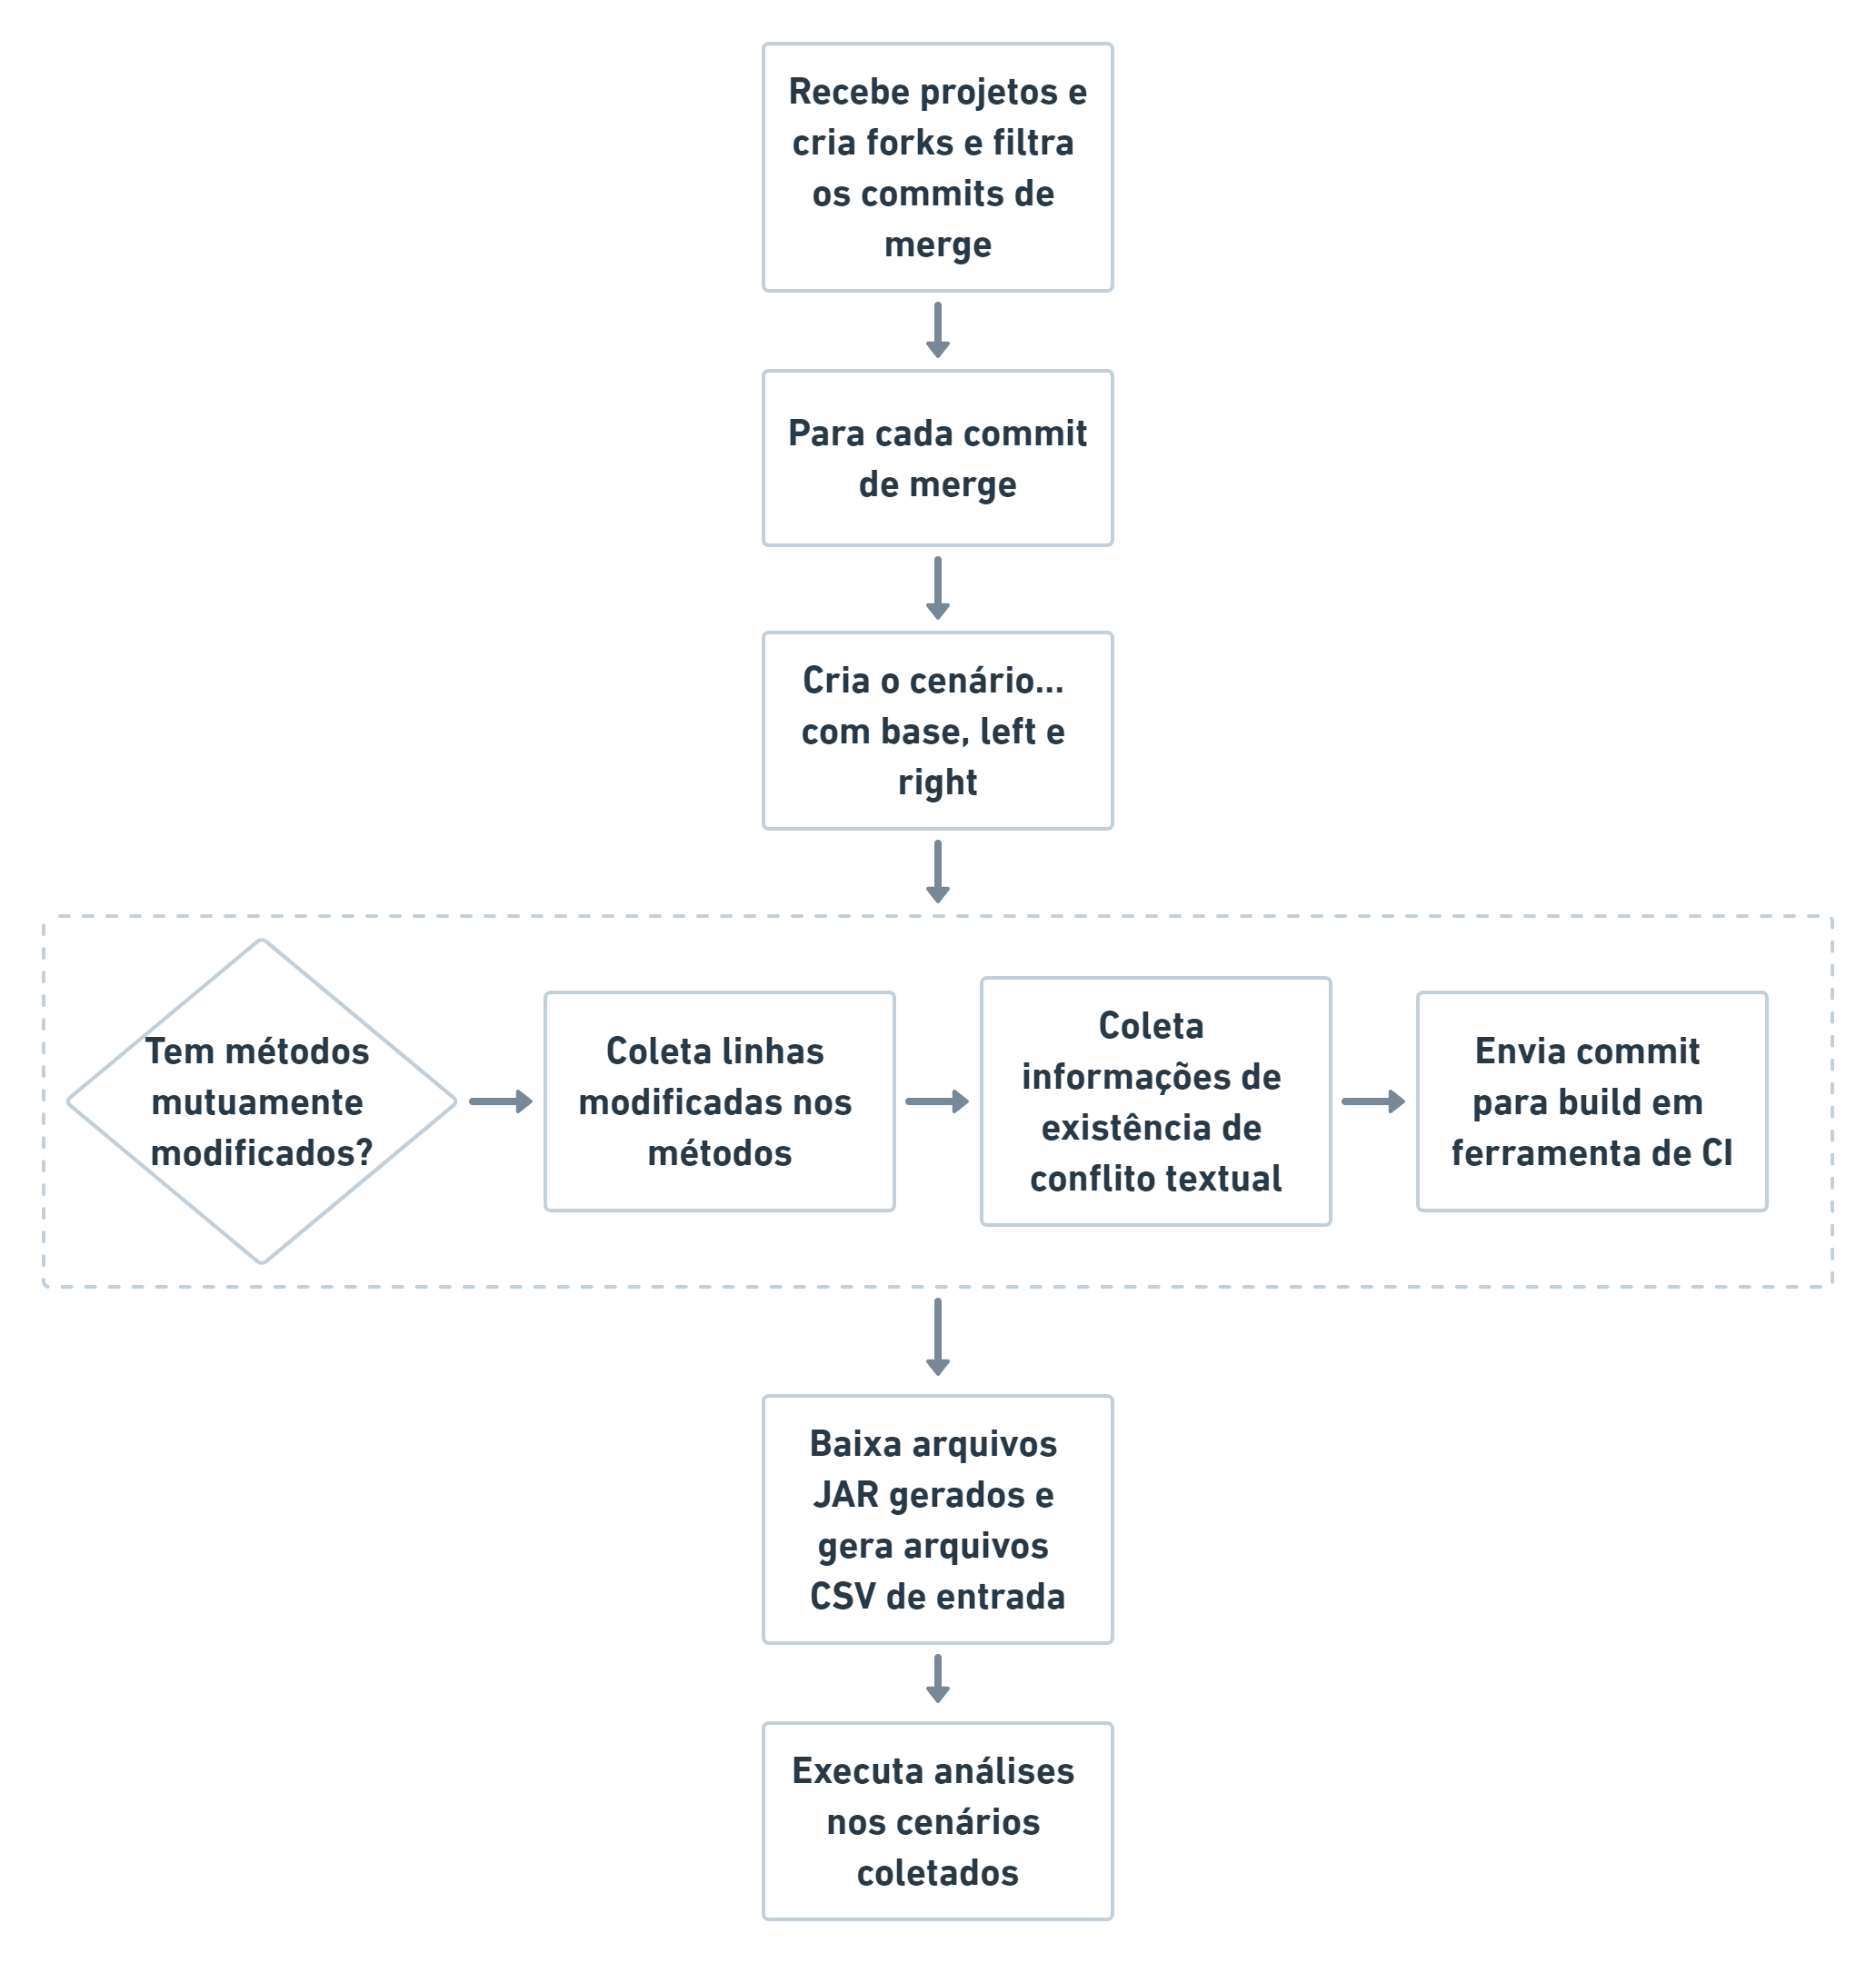
\includegraphics[width=0.8\linewidth]{samples/images/Fluxo de mineracao.png}
    \caption{Fluxo de coleta dos dados sobre os cenários de integração}
    \label{fig:mineracao}
\end{figure}

Para cada \emph{commit}, a ferramenta primeiro checa se existem métodos ou atributos de classe modificados por ambas as versões \emph{Left} e \emph{Right}, caso não existam, o \emph{commit} é ignorado. Caso existam, a ferramenta continua o processo de coleta de dados: coleta os números das linhas das modificações de \emph{Left} e \emph{Right}, faz o replay do \emph{merge} e depois verifica a existência de conflitos de integração textuais e registra em uma planilha. Por fim, envia o cenário para geração dos arquivos \emph{JAR} em uma ferramenta de CI. A ferramenta gera um arquivo de configuração para a plataforma de CI \emph{Github Actions}\footnote{Um exemplo de arquivo gerado para um projeto real (jsoup) pode ser visto em: https://gist.github.com/barbosamaatheus/073dc8caa24e3e775e2483629c476856.
}, que usa os sistemas de \emph{build} \emph{Maven} ou \emph{Gradle} para gerar os arquivos JAR.


O Processo supracitado foi utilizado na maioria dos casos, no entanto, em alguns desses cenários, o mapeamento das linhas do código-fonte extraídos a partir do \emph{bytecode}, pode ser impreciso, por isso precisaram passar por adaptações, assim dizemos que eles são realistas. Esse problema ocorre principalmente nos casos em que há chamadas de método encadeadas que ocupam várias linhas. Isso está ligado ao modo como a associação do número da linha é armazenada no arquivo de classe (\emph{.class}) e no histórico do compilador \emph{javac}. Para evitar esses comandos que ocupam várias linhas, quebramos o mesmo em vários comandos que ocupam apenas uma linha, através de simples refatorações de extrações de variáveis no código-fonte do projeto para que o comportamento original do programa fosse preservado, mas que o \emph{bytecode} tivesse o mapeamento esperado das linhas. Esse tratamento foi aplicado em três cenários.

Para a análise de cenários cujo método de entrada tinha pelo menos um argumento com tipo não primitivo, adicionamos um método que instancia os parâmetros e chama o método de entrada. Essa estratégia foi aplicada em quatro cenários e usada apenas pela implementação \emph{intraprocedural} e foi necessária, pois a análise não reconhece parâmetros de tipos não primitivos que não foram instanciados previamente no código. 

Após executar o processo descrito anteriormente, para cada um dos \emph{commits} de \emph{merge}, a ferramenta baixa os arquivos \emph{JAR} gerados na plataforma de CI e gera os arquivos de entrada para a execução da análise de OA.

Todos os arquivos utilizados para avaliação, assim como as instruções para gerar os arquivos \emph{JAR} que foram gerados manualmente, podem ser encontrados no projeto \href{https://github.com/spgroup/mergedataset}{mergedataset}\footnote{Este repositório agrupa um conjunto de cenários de mesclagem com conflitos semânticos conhecidos, coletados de estudos relacionados. https://github.com/spgroup/mergedataset}. Um resumo da amostra utilizada pode ser observada no Apêndice Online \rev{\cite{sitesbes2022}}.

\subsection{Metodologia}
\label{sec:metodologia}

A \hyperref[fig:fluxo-execucao]{Figura 9} apresenta o fluxo de trabalho seguido no estudo empírico.

\begin{figure}[!h]
    \centering
    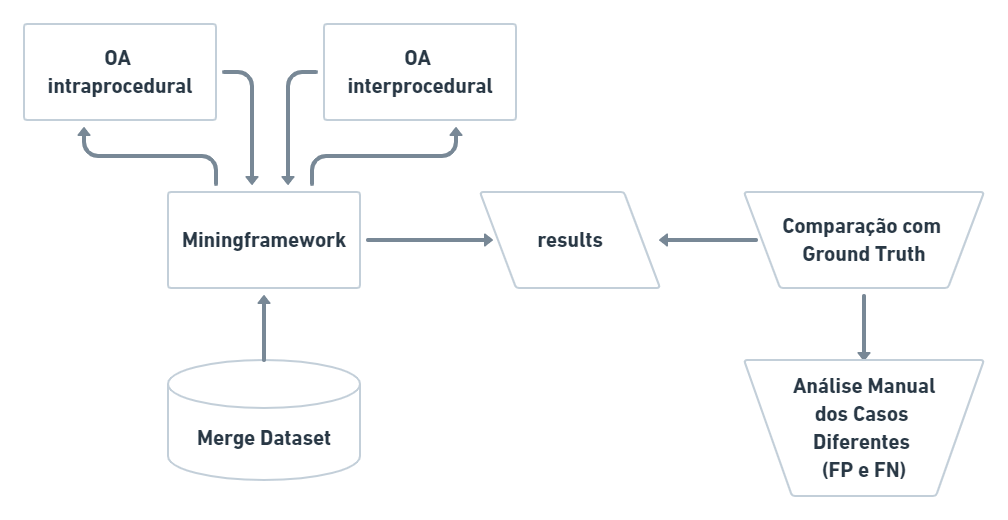
\includegraphics[width=0.8\linewidth]{images/Fluxo da avaliação.png}
    \caption{Fluxo da execução da avaliação das análises.}
    \label{fig:fluxo-execucao}
\end{figure}


Com os dados necessários para os 78 cenários, o \href{https://github.com/spgroup/miningframework}{miningframework} foi utilizado para executar as implementações  \emph{intraprocedural} e  \emph{interprocedural} em cada um dos cenários. Para fins de avaliação, o resultado de uma análise é considerado positivo para um cenário específico se a execução retornar uma ou mais interferências.

Todos os 78 cenários do conjunto de dados também foram analisados manualmente, utilizando o protocolo disponível no Apêndice Online \rev{\cite{sitesbes2022}}, de modo a verificar a existência de interferências entre as modificações de \emph{Left} e \emph{Right}, e assim estabelecer um \emph{Ground Truth}. Para definição do \emph{Ground Truth}, foi usado um processo estruturado de checagem dupla, onde cada cenário foi atribuído a dois colaboradores que realizaram a análise de forma individual registrando justificativas para suas decisões. A análise individual dos dois colaboradores foi comparada, e caso o resultado convergisse, o mesmo seria adotado com \emph{Ground Truth} do cenário. Em caso de divergência, os colaboradores se reuniam e discutiam o cenário, buscando chegar a um consenso. Nos casos em que o consenso não foi atingido, o cenário era apresentado a outro colaborador para juntos chegarem 
à decisão.

Buscando verificar a capacidade da análise em detectar interferência entre as contribuições ou até mesmo compor uma ferramenta para detecção de conflitos de integração semânticos mais robusta, os resultados apresentados pelas implementações da análise proposta foram comparados com o \emph{Ground Truth} em cada cenário. Adicionalmente, para verificarmos o quão próximo a nossa implementação atual está de uma implementação ideal de OA, comparamos o resultado da ferramenta com \emph{Ground Truth} exclusivo de OA. 

Por fim, foi realizada uma análise manual dos casos diferentes (Falsos Positivos e Falsos Negativos) onde foi possível identificar os motivos pelos quais a análise não produziu o resultado esperado.\footnote{Feita apenas para a abordagem \emph{interprocedural}} Isso não é o objetivo principal deste trabalho, assim como a otimização da implementação e a avaliação da métrica de tempo. Desta forma, não aprofundamos esses itens, mas pretendemos realizar em trabalhos futuros, assim como a análise dos casos positivos, onde verificaremos se os alertas gerados pela análise correspondem às interferências detectadas na análise manual.

\subsection{Resultados}

\subsubsection{Resultados Reportados nas Execuções das Implementações da Analíse}

Ao executar a abordagem \emph{intraprocedural} da análise proposta para 78 cenários do \emph{dataset} obtivemos 13,2\% de casos reportados como verdadeiros, ou seja, a análise reportou pelo menos uma interferência nesses cenários. Em 80,9\% dos casos, a análise não detectou nenhuma interferência. Ainda foram reportados 4 casos (5,9\%) que não foram encontrados pela análise, isso ocorreu, pois, esses cenários tinham apenas remoções de linhas feitas pelo desenvolvedor \emph{Right}. Outros 10 casos apresentaram erro na execução. Os casos com erro ou que não foram encontrados foram desconsiderados para fins de comparação com o \emph{ground truth}.

Já a execução \emph{interprocedural} também reportou os mesmos 4 casos (5,1\%) como não encontrado. Além disso, apresentou 6 casos (7,7\%) em que a análise foi interrompida por exceder o limite de tempo\footnote{O  \emph{timeout} pode acontecer, pois, devido à característica da abordagem \emph{interprocedural} que acessa e analisa o corpo de todos os métodos chamados nós próprios métodos analisados, o que exige um tempo maior de execução por isso é definido um tempo limite que quando é atingido, para a execução da análise e retorna um status de \emph{timeout}.} estipulado para cada cenário. Esses 10 casos, foram desconsiderados para fins de comparação com o \emph{ground truth}. A execução \emph{interprocedural} também reportou 15.4\% dos casos como verdadeiros e 71,8\% como falso.

\subsubsection{OA x Análise Manual de LOI}

Os resultados apresentados nessa subseção foram obtidos comparando os resultados da execução das implementações da análise proposta com o \emph{Ground Truth} para interferência localmente observável. Essa comparação pretende avaliar o algoritmo para detecção de interferências entre as contribuições das versões integradas, portanto, para detecção de conflitos semânticos.

\begin{figure}[!h]
    \centering
    \includegraphics[width=0.9\linewidth]{images/OA x Análise Manual de LOI.png}
    \caption{Resultados da análise em comparação com o \emph{Ground Truth} de LOI.}
    \label{fig:loi-x-groundtruthloi}
\end{figure}

Os resultados ilustrados na \hyperref[fig:loi-x-groundtruthloi]{Figura 10} mostram a comparação dos 64 cenários considerados na execução \emph{intraprocedural} com o \emph{ground truth} de LOI. Obteve-se uma taxa alta de 34,4\% de falsos negativos e 7,8\% de falsos positivos. Logicamente, os outros 57,9\% foram de acertos da ferramente, sendo 51,6\% verdadeiros negativos e 6,3\% de verdadeiros positivos. 

Ainda na \hyperref[fig:loi-x-groundtruthloi]{Figura 10}, conseguimos observar também os resultados da comparação dos 68 cenários considerados na execução \emph{interprocedural} com o \emph{ground truth} de LOI. Obtendo-se uma taxa de 27,9\% de falsos negativos e 7,4\% de falsos positivos. os outros 64,7\% foram de acertos da ferramente, sendo 54,4\% verdadeiros negativos e 10,3\% de verdadeiros positivos.

A \hyperref[tab:erros-inter-loi]{Tabela 1} apresenta um sumário com a descrição e a quantidade de erros da análise \emph{interprocedural} proposta.

\begin{table}[h]
    \centering
    \begin{tabularx}{\linewidth}{X c c}
        \hline
        Descrição do Cenário (em relação à causa do erro) & \multicolumn{1}{l}{Quantidade} & \multicolumn{1}{l}{Tipo de erro} \\ \hline
        String com mais de uma linha é alterada em linhas diferentes & 1 & FN \\ \hline
        Alterações apenas na inicialização de atributos que possuem mais de uma linha & 2 & FN \\ \hline
        \emph{Callgraph} não consegue encontrar possíveis classes de destino, pois faltam dependências & 2  & FN \\ \hline
        Interferência não é detectável com OA & 14 & FN \\ \hline
        Não existe interferência entre as contribuições & 5  & FP\\ \hline
    \end{tabularx}
    \caption{Descrições dos cenários em que a análise \emph{interprocedural} proposta errou na detecção de LOI.}
    \label{tab:erros-inter-loi}
\end{table}

Os dois últimos itens da tabela já são esperados, pois, a análise foi projetada para detectar OA e como já dito anteriormente a existência de OA não implica necessariamente na existência de LOI e vice-versa.

O primeiro caso da tabela pode ser observado na imagem ilustrada na \hyperref[fig:ad2be67]{Figura 11}. Para esse caso temos que \emph{Left} e \emph{Right} alteraram a \emph{String} que vai ser usado no retorno da função. O \emph{ground truth} classifica isso como OA, no entanto, ao nível de execução da implementação da análise, o \emph{Soot framework} vai gerar variáveis temporárias para cada uma das linhas, dessa forma a análise não consegue associar as mudanças feitas pelos desenvolvedores a mesma variável. Isso é uma limitação da implementação que pretendemos resolver em trabalhos futuros.

\begin{figure}[h]
    \begin{lstlisting}[escapechar=!]
    @Override
    public String toString()() {
        return "KafkaSpoutConfig{" +
        ", k!\colorbox{yellow}{eys" + getK}!eyDeserializer!\colorbox{yellow}{() +}!
        ", value=" + !\colorbox{yellow}{getV}!alueDeserializer!\colorbox{yellow}{()}! +
       ...
        !\colorbox{green}{   }!
        ...
        '}';
    }
    \end{lstlisting}
    \caption{\rev{Cenário Storm ad2be67 no método toString() como exemplo para o falso negativo.}}
    \label{fig:ad2be67}
    \centering
\end{figure}

A partir dos resultados das execuções das implementações da análise foram calculadas as métricas representadas pela \hyperref[tab:metrics-loi]{Tabela 2}.

Para a métrica de precisão, a análise \emph{interprocedural} obteve o valor de 0,6, enquanto a análise \emph{intraprocedural} proposta tem uma precisão de 0,4. Os valores são bem próximos e indicam que alguns dos casos indicados como positivos foram classificados corretamente, mas também que grande parte dos casos indicados como positivos foram classificados incorretamente. A quantidade de falsos positivos é esperada, pois, existem casos em que existe OA,
mas \emph{Ground truth} de LOI é falso, desta forma as implementações vão detectar OA, mas não existe interferência real. Um exemplo disso acontece um dos desenvolvedores fez apenas uma refatoração estrutural no código.

Para a métrica de revocação, a análise \emph{interprocedural} obteve o valor de 0,3, enquanto a análise \emph{intraprocedural} obteve 0,2. Novamente os valores são muito próximos e indicam que a maioria dos casos positivos não são detectados pelas abordagens. A priori, esses números podem parecer baixos, no entanto, a principal razão para isso está em nossa amostra que contém diversos tipos de interferência, como, por exemplo, casos em que um desenvolvedor escreve em uma variável que outro desenvolvedor futuramente lê. Esses tipos diferentes de interferência não são detectados pelo algoritmo de OA que busca apenas variáveis atribuídas por dois desenvolvedores diferentes. A combinação da análise de OA com outras análises melhoraria consideravelmente os resultados de revocação. Além disso, a solução dos problemas e limitações conhecidas nas implementações atuais, colocaria os resultados de revocação em seu nível máximo. 

A análise \emph{interprocedural}, por sua característica e natureza, tem uma acurácia melhor por ser uma análise menos sensível e detectar mais casos positivos que a análise \emph{intraprocedural}, isso fica comprovado no resultado onde a análise \emph{interprocedural} teve uma acurácia de 0,64, enquanto a \emph{intraprocedural} recebeu 0,57. De modo geral, os resultados para essa métrica são considerados bons, mas podem ser significativamente melhorados aplicando principalmente as soluções supracitadas para melhoria da revocação.

\begin{table}[!h]
    \centering
    \begin{tabular}{ l  l  l }
        \hline
                  & Intraprocedural & Interprocedural  \\
        \hline
        Precisão & 0,4 & 0,6 \\
        \hline
        Revocação & 0,2 & 0,3 \\
        \hline
        Acurácia  & 0,57 & 0,64 \\
        \hline
        
    \end{tabular}
    \caption{Resultados das Métricas para a detecção de LOI}
    \label{tab:metrics-loi}
\end{table}

Comparando os resultados das duas execuções, podemos observar resultados semelhantes com uma leve vantagem para a abordagem \emph{interprocedural}. Isso é esperado, pois a \emph{interprocedural} percorre e analisa uma quantidade maior de código-fonte, o que faz com que ela consiga sinalizar casos adicionais de interferência. No entanto, pelo mesmo motivo, o custo de execução \emph{interprocedural} é maior. Isso faz com que a abordagem \emph{intraprocedural} seja ainda mais relevante. 

Em geral, podemos concluir que a análise proposta consegue detectar interferência entre as modificações em um cenário de integração, o que pode indicar que ela é uma boa ferramenta para detecção de conflitos de integração semânticos. No entanto,  existem outros tipos de cenário de interferência que análises OA não é capaz de detectar, o que indica que somente a análise proposta não é suficiente para ser utilizada sozinha, como uma ferramenta confiável para detecção de conflitos semânticos. A análise proposta poderia ser combinada com outras análises que buscam detectar outros tipos de interferência para criar uma ferramenta mais robusta. Análises de OA podem errar na detecção de interferência e com a análise proposta não é diferente. Nesse  sentido, uma ferramenta com suporte a OA pode ser muito sensível e apresentar falsos positivos e falsos negativos.

\subsubsection{OA x Análise Manual de OA}

Os resultados apresentados nessa subseção foram obtidos comparando os resultados da análise proposta com o \emph{Ground Truth} para OA. Essa comparação visa avaliar a capacidade da análise proposta para detecção da existência de substituição de atribuições (OA) entre as contribuições de dois desenvolvedores em um cenário de integração de código. Através dessa comparação, podemos identificar a qualidade das implementações atuais e o quão perto elas estão de uma implementação ideal de OA.

A partir dos resultados obtidos através da execução das implementações da análise foram calculadas as métricas representadas pela \hyperref[tab:metrics-oa]{Tabela 3}.

\begin{table}[!h]
    \centering
    \begin{tabular}{ l  l  l }
        \hline
        & Intraprocedural & Interprocedural  \\
        \hline
        Precisão & 0,44 & 1.0 \\
        \hline
        Revocação & 0,22 & 0,6 \\
        \hline
        Acurácia  & 0,7 & 0,88 \\
        \hline
        
    \end{tabular}
    \caption{Resultados das métricas para a detecção de OA}
    \label{tab:metrics-oa}
\end{table}

A análise proposta se mostrou capaz de detectar cenários com substituições de atribuições entre as contribuições, principalmente na sua abordagem \emph{interprocedural}. No entanto, a análise reportou falsos positivos e falsos negativos. O número de falsos positivos foi baixo e isso indica que a análise reporta poucos "alarmes falsos", gerando um custo pequeno para o desenvolvedor, que não vai ser distraído facilmente por problemas que não existem de fato. Os falsos negativos estão associados a limitações da análise, e acontecem, por exemplo, quando as modificações introduzidas pelos desenvolvedores estão em inicializações de atributos com múltiplas linhas e não existe um método de entrada. 

Com isso concluímos que a análise apresentou excelentes índices, princialmente na métrica de  acurácia. (0,7\% para \emph{intraprocedural} e 0,88\% para \emph{interprocedural}). Isso significa que as implementações atuais precisam de poucos ajustes para se tornarem ideias no sentido de detecção de OA.

\subsubsection{Detalhes da execução}
Embora o desempenho não fosse uma prioridade para nosso projeto, deixamos aqui os registros dos dados coletados relacionados ao tempo de execução da análise.

As duas abordagens da análise foram executadas utilizando uma máquina virtual com sistema operacional Linux Ubuntu 20.04.2 LTS 64-bit, 4 \emph{Gigabyte} de memória RAM, processador Intel® Core™ i5-9300H CPU @ 2.40GHz × 4. Ambas tiveram o \emph{timeout} configurado em 240 segundos. A execução \emph{interprocedural} foi configurada com um limite de profundidade no acesso aos métodos de 5. 

Com dados de uma execução e tomando a média dos tempos medidos, a execução \emph{intraprocedural} levou 2,32 segundos/por cenário para analisar toda a amostra, com mediana de 1,09 e desvio padrão de 2,42.  Já a execução \emph{interprocedural} teve media de 28,12 segundos/por cenário, mediana de 3,94 e desvio padrão de 68,81.

Analisando os resultados podemos perceber que a abordagem \emph{interprocedural} é consideravelmente mais lenta em relação à média de tempo por cenário do que a abordagem \emph{intraprocedural}. Isso é esperado, pois, como a \emph{intraprocedural} tem como característica, ignorar as chamadas de método no método de entrada, ela percorre um caminho mais curto durante a execução. O contrário ocorre na execução \emph{interprocedural} que permite acessar e analisar todo o corpo de todas as chamadas de método até que o seu limite de profundidade, definido por parâmetro, seja atingido. Utilizando o referencial dos resultados atuais, indicamos a implementação \emph{interprocedural} pois a mesma obteve resultados melhores na detecção de interferência, mas devido ao seu custo maior, acreditamos que a mesma possa ser utilizada em rotinas que executam à noite, por exemplo. Para contextos onde o tempo é um fator limitante a implementação \emph{intraprocedural} é a mais recomendada. 

É importante ressaltar que as implementações utilizadas nesse trabalho são protótipos e não foram otimizadas visando desempenho, uma vez que o objetivo era verificar a capacidade da mesma em detectar interveniências. Com isso, queremos dizer que os resultados de desempenho podem ser substancialmente melhorados.  

\subsection{Ameaças a validade}

Nosso estudo se restringe à ocorrência de interferência local. Portanto, é possível que nossos exemplos tenham cenários de \emph{merge} que as alterações não interferem umas com as outras localmente, mas interferem globalmente. O contrário também pode ocorrer. Então o número de falsos negativos e falsos positivos em relação a uma noção de interferência pode diferir do nosso relatório de resultados.



Além disso, ao definir o \emph{ground truth}, conhecer os resultados da análise proposta antes da análise manual pode ter influenciado o veredicto. Por exemplo,
sabendo que a ferramenta não foi bem sucedida para um determinado cenário traz o risco de impedir uma análise manual mais aprofundada. Para reduzir essa ameaça, envolvemos dois autores na definição de \emph{ground truth}, e exigiu-se que eles fornecessem uma explicação de porque não há interferência. 

\rev{O tipo de cenário contido no nosso dataset, com mudanças em paralelo no mesmo método ou atributo pode ser mais suscetível a ocorrência de interferência, mas isso não influencia o resultado final principal apresentado no artigo sobre a acurácia e performance de uma ferramenta baseada na análise OA, já que no dataset temos vários casos de interferência, mas também vários casos sem interferência, e nossa avaliação principal não é sobre a frequência com que interferência ocorre, mas sim se análise estática seria viável para detectar interferência. Adotamos esse critério de filtro dos cenários de merge para reduzir um pouco a dificuldade de analisar manualmente cenários reais para confirmar a ocorrência de interferência. Nenhum outro filtro sobre o conteúdo dos métodos e atributos dos cenários foi aplicado.}

O objetivo principal deste trabalho é verificar a utilidade da análise proposta em detectar interferências entre as contribuições. Com isso, não investimos na otimização das implementações da análise, o que pode fazer com que a implementação atual apresente erros. Alguns problemas conhecidos já foram mencionados, mas podem existir outros problemas que ainda não foram detectados. 
Alguns dos cenários do \emph{dataset} utilizado precisaram de adaptações realistas. Essas alterações foram realizadas no código-fonte de sete cenários buscando manter o máximo das características originais. No entanto, essas alterações foram feitas de forma manual e não foram executados testes para validar que o comportamento original foi mantido, no entanto, deixamos o alerta que esses casos são tratados como cenários realistas e não reais de fato.


\section{Trabalhos relacionados}
Nesta seção descrevemos alguns dos estudos anteriores que usamos como base de evidência para nosso estudo e trabalhos relacionados.

Vários pesquisadores já investigaram sobre os conflitos de \emph{merge} e como eles afetam os desenvolvedores e a produtividade de forma geral \cite{10.1145/383876.383878, 4228648, Sarma, Bird2012AssessingTV, 8094445, 6915251, 9625780, 10.5555/1781794.1781836}. Em contraste, aqui focamos na detecção de conflitos semânticos, que normalmente são mais difíceis de se detectar e resolver. Não conhecemos trabalhos que analisam o impacto de conflitos semânticos em produtividade. No entanto, ferramentas como a que discutimos aqui são essenciais para ajudar a entender o impacto de conflitos semânticos em produtividade.

%Pesquisadores também analisaram outras maneiras de detectar ou prevenir conflitos, minimizando assim o impacto na produtividade. Sarma et al. \cite{Sarma} apresenta uma ferramenta projetada para reduzir conflitos, notificando os desenvolvedores sobre mudanças paralelas no mesmo artefato. Com esse intuito, existem também outras ferramentas.  \cite{10.1145/1810295.1810339, DBLP:journals/corr/abs-1105-0768, 10.5555/2486788.2486884, 10.1145/2675133.2675177,10.1145/2950290.2950339,10.1007/s10515-017-0227-0, Klissiomara, 10.1145/3238147.3241983, 6475431, 1000449}.

Com o intuito de progredir no processo de detecção de conflitos de \emph{merge} de forma mais precisa e reduzir esforços da integração, foram criadas diversas ferramentas. Westfechtel \cite{10.1145/111062.111071} e Buffenbarger \cite{Buffenbarger} foram pioneiros em propor soluções para realizar \emph{merge} usando estruturas de arquivos. Posteriormente, outros pesquisadores implementaram soluções baseadas em construções específicas de linguagens de programação, como \emph{Java} \cite{10.1007/s10515-006-0002-0} e \emph{C++} \cite{Cdiff}.
Existem também várias ferramentas de \emph{merge} avançadas que usam a estrutura sintática dos programas integrados \cite{10.1145/2025113.2025141, 7321191, 10.1145/3133883, 8952450, 6494912, 10.1109/ICSE-Companion.2019.00117, 10.1109/ASE.2019.00097, 10.1145/3474624.3474646}, mas nenhuma delas captura conflitos semânticos dinâmicos como os ilustrados aqui.

Para de fato detectar conflitos semânticos, Da Silva \emph{et al} \cite{LeusonSilva2020} propuseram uma abordagem baseada em geração de testes unitários automatizados como especificações parciais para detecção de interferência em cenários de integração. Com 38 cenários testados, a abordagem conseguiu detectar 4 casos com conflitos (verdadeiros positivos), 11 casos falsos negativos (28,95\%) e nenhum falso positivo. Já em nosso trabalho, utilizamos uma abordagem diferente, baseada em análise estática. Os resultados para os 78 cenários da amostra utilizada apontam um percentual maior de falsos positivos (7,8\% para \emph{intraprocedural} e 7,4\% para \emph{interprocedural}) e falsos negativos (34,4\% para \emph{intraprocedural}). A nossa abordagem foi superior na comparação de falsos negativos \emph{interprocedural} (27,9\%). Contudo, argumentamos que a análise proposta neste trabalho é somente uma parte de uma solução maior utilizando analises estáticas, enquanto o trabalho de Da Silva é uma solução completa. A amostra de 38 cenários utilizada no trabalho de testes é um subconjunto da amostra utilizada em nosso trabalho. Nesse sentido, analisamos os cenários detectados por ambas as ferramentas e constatamos serem cenários diferentes. Dessa forma, entendemos que uma combinação das duas abordagens poderia ser usada em trabalhos futuros, buscando aumentar a quantidade de cenários detectados e reduzir o número de erros, principalmente os falsos negativos. Além disso, existem outros trabalhos importantes que seguem a linha de ferramentas baseadas em testes \cite{brun, 10.1145/2786805.2803208, 10.1145/2568225.2568300}, mas estes são baseados em testes do projeto, que muitas vezes não são suficientes para detectar conflitos.

Por fim, ferramentas baseadas em estratégias de análise estática também foram propostas \cite{10.1145/201055.201056, 10.1145/65979.65980, 336770, 10.1145/131736.131756, Horwitz1989IntegratingNV, 10.1145/3276535, 1113835899}. Barros Filho \cite{InformationFlowRoberto} também propôs a utilização de análises com o objetivo principal de entender se o Information Flow Control (IFC) pode ser utilizada para indicar a presença de conflitos semânticos dinâmicos entre as contribuições dos desenvolvedores em cenários de \empty{merge}. Essa análise se mostrou capaz de detectar casos de interferência, porém com uma taxa de 57.14\% de falsos positivos. Contudo, a análise implementada utilizava um grafo complexo para representar as dependências entre unidades do código, o que faz com que a análise consuma muitos recursos computacionais. Em nosso trabalho, apresentamos uma análise mais simplificada que busca detectar apenas conflitos de OA. Avaliamos a análise proposta utilizando uma amostra maior do que o dobro da amostra de Barros Filho e obtivemos um número de falsos positivos cerca de 87\% menor.
\section{Conclusões}

Neste estudo apresentamos uma proposta de análise estática de substituição de atribuições entre contribuições de dois desenvolvedores, de modo a detectar interferencias. Foi implementado duas abordagens para a análise proposta, sendo uma \emph{intraprocedural} e outra \emph{interprocedural}.

\rev{Apesar de haver outros tipos de análise que podem detectar interferência, focamos em OA por ela ter mais chances de ser efetiva, já que a nossa expectativa era de que normalmente quando há esse tipo de sobreposição há também interferência. Além disso, existe a necessidade de entender com precisão os pontos fortes e fracos de cada análise individualmente de forma a poder sugerir uma combinação de análises que seja mais efetiva para detectar interferência.}

A análise proposta se mostrou capaz de detectar cenários com substituições de atribuições e com interferência localmente observável entre as contribuições. No entanto, teve uma quantidade considerável de falsos negativos, o que indica que ela não é suficiente para detectar cenários com interferência de forma confiável. Portanto, a análise proposta poderia ser combinada com outras para compor uma ferramenta mais robusta para detecção de conflitos de integração semânticos.

\rev{Como trabalho futuro, pretende-se implementar a resolução de algumas limitações conhecidas para a análise, além de realizar combinações com outras ferramentas de detecção de conflitos semânticos relacionadas.}
\rev{\section*{Disponibilidade de Artefatos}
Disponibilizamos o código-fonte das implementações da análise, o \emph{dataset} utilizado na avaliação, uma planilha com os resultados das execuções, um documento com o protocolo utilizado para definição de \emph{Ground Truth} e instruções de replicação do estudo \cite{sitesbes2022}.}
\rev{\section*{Agradecimentos}
Agradecemos Rafael Alves, Léuson Santos e Vinícius dos Santos pelo suporte na hora de criar nosso conjunto de dados. Agradecemos também INES (Instituto Nacional de Engenharia de Software) e FACEPE (IBPG-0028-1.03/20 e IBPG-0567-1.03/22).}

% \cleardoublepage
% \phantomsection
\addcontentsline{toc}{chapter}{Referências Bibliográficas}
\nocite{*}
\bibliographystyle{plain}
\bibliography{biblio}

%\appendix

% \include{appendix}

\end{document}
\endinput
%%
%% End of file `sample-sigconf.tex'.
